\documentclass[12pt]{article}

\usepackage{amsmath}    % need for subequations
\usepackage{graphicx}   % need for figures
\usepackage{verbatim}   % useful for program listings
\usepackage{color}      % use if color is used in text
\usepackage{subfigure}  % use for side-by-side figures
\usepackage{hyperref}   % use for hypertext links, including those to external documents and URLs

\setlength{\baselineskip}{16.0pt}    % 16 pt usual spacing between lines
\setlength{\parskip}{3pt plus 2pt}
\setlength{\parindent}{20pt}
\setlength{\oddsidemargin}{0.5cm}
\setlength{\evensidemargin}{0.5cm}
\setlength{\marginparsep}{0.75cm}
\setlength{\marginparwidth}{2.5cm}
\setlength{\marginparpush}{1.0cm}
\setlength{\textwidth}{150mm}

\begin{comment}
\pagestyle{empty}
\end{comment}



\begin{document}

\begin{center}
{\large Hybrid Partitioning in Zoltan} \\
Nick Aase,  Karen Devine \\
Summer, 2011
\end{center}


\section{Introduction}
When used for partitioning, Zoltan has a wide range of algorithms
available to it. Traditionally they have fallen into two categories:
geometric-based partitioning, and topology-based partitioning. Each
method has its own strengths and weaknesses which ultimately come down
to the tradeoff between speed and quality, and the onus is placed
upon the user to determine which is more desirable for the project
at hand.

In our project we strived to develop a hybrid partitioning algorithm;
one that attempts to take advantage of the efficiency of geometric
methods, as well as the precision of topological ones. The reasoning
behind this concept is that problem sets with large amounts of data may
be more easily digestible by topological methods if they are first
reduced into managable pieces based on their geometry.

The two subjects chosen for this project were the Recursive
Coordinate Bisection (RCB) algorithm and Parallel Hypergraph
partitioning (PHG). RCB is an extremely fast method of partitioning,
but it can be clumsy at times when it ``cuts'' across a coordinate plane.
On the other hand, PHG has a good understanding of the relationships
between data, making its partitioning quite accurate, but it suffers
from having to spend a great deal of time finding those relationships.

For further information on implementing hybrid partitioning, please see
the developer's guide at
http://www.cs.sandia.gov/Zoltan/dev\_html/dev\_hybrid.html


\section{Parallel hypergraphs and geometric input}
In order for Zoltan to support hybrid partitioning, it is necessary
to properly and frequently obtain, preserve, and communicate coordinate
data. The first step that needed to be taken was to modify PHG to
support coordinate information. Hypergraph objects carry a substantial
amount of data already, but we had to add an array of floating point
values to store the coordinates. Currently, when a hypergraph is built and
geometric information is available from the input, each vertex will have
a corresponding subset within the array defining its coordinates;
that is, \forall\, $v_x$\in\, $H:$\, \exists\, $C_x =  \{c_0, c_1, ..., c_{n-1}\},$
where $v_x$ is an arbitrary vertex in the hypergraph $H$, $C_x$ is its
corresponding coordinate subset, and $n$ is the number of dimensions in
the system. In this way, Zoltan can treat each coordinate subset as an
element of that vertex


\section{PHG, MPI and 2-dimensional representation}
PHG is interesting in that multiple processors can share partial data
that describes the properties of hyperedges and vertices. This sort of
system can be represented in a 2-dimensional distribution similar to
Table 1. A populated field represents that a processor on the y-axis has
data related to the vertex on the x-axis. In this example, you can see
that processor $P_0$ and $P_2$ share data describing vertices $v_0$ and
$v_2$.

\begin{table}[h]
\begin{center}
\begin{tabular}{|r|l|l|l|}
  \hline
  Processor & $v_0$ & $v_1$ & $v_2$ \\
  \hline
  $P_0$ & x &   & x \\
  \hline
  $P_1$ &   & x &   \\  
  \hline
  $P_2$ & x &   & x \\
  \hline
\end{tabular}
\caption{\label{tab:0/tc} Before communication}
\end{center}
\end{table}

Using Message Passing Interface (MPI) communicators, it is possible to
communicate with processors by column. We use an \texttt{MPI\_Allreduce}
call to collect data from each processor, which groups them into a usable
form. Consider Table 2.

\begin{table}[h]
\begin{center}
\begin{tabular}{|r|l|l|l|}
  \hline
  Processor & $v_0$ & $v_1$ & $v_2$ \\
  \hline
  $P_0$ & x &   &   \\
  \hline
  $P_1$ &   & x &   \\  
  \hline
  $P_2$ &   &   & x \\
  \hline
\end{tabular}
\caption{\label{tab:1/tc} After communication}
\end{center}
\end{table}

This same sort of operation is performed with weight data, so implementing
it on coordinate data was simply another step in setting up PHG to support
coordinate information from the input. Afterwards the entirity of a vertex's
data will be unique to a single processor, with the number of global
vertices == $\sum_{i=0}^{numProc-1} ($number of local vertices_i$)$.


\section{Matching}
There are several matching methods already native to Zoltan and specific to
PHG, but we needed to create a new method in order to use RCB on the
hypergraph data. Before the actual matching occurs several specialized
callbacks and parameters are registered. Doing this is crucial if RCB and PHG
are to interface properly with each other.

The next task is to physically call RCB. It was easy enough to send PHG
data to RCB as we simply used the \texttt{Zoltan\_LB\_Partition} wrapper,
not unlike other standard load balancing partitioners. However, getting
matchings \emph{back} from RCB to PHG was another matter entirely. Thanks to
Dr. Devine's work, we were able to ostensibly comondeer one of RCB's unused
return values: since all matching algorithms conform syntactically to the
afforementioned load-balancing wrapper, there are some arguments and/or
values that are never used depending on what data that partitioner needs In
the case of RCB, the return value \texttt{*export\_global\_ids}, which is
defined in its prototype, was never actually computed. Dr. Devine was able
to rewire RCB so that, when using hybrid partitioning, it would return the
IDs of the matchings we need for each hypergraph (which are referred to in
the matching procedure as \emph{candidates}).

This new matching procedure is similar to PHG's agglomerative matching,
whereby candidate vertices are selected to represent groups of similar
vertices. These candidates then make up the standard vertices in the
resultant coarse hypergraph. The major difference is that standard
agglomerative matching determines its candidates by the connectivity of
vertices to one another; the more heavily connected a subset of vertices
is, the more likely they will share the same candidate. Using RCB means
making the assumption that related vertices will be geometrically similar:
recursive geometric cuts will be more likely to naturally bisect less
connected parts of the hypergraph, and the vertices that are members of
the resulting subdomains will share the same candidates. Given RCB's
track record, this method should be significantly faster than the
agglomerative matching.


\section{Reduction factor}
When using hybrid partitioning, the user passes a parameter in the input
file called \texttt{HYBRID\_REDUCTION\_FACTOR}, which is a number $> 0$
and $\leq 1$ that gets passed into RCB. This parameter defines the
aggressiveness of the overall procedure. This number simply determines
the amount by which the larger graph will be reduced (e.g. for the
original, fine hypergraph, $H_f$, where the number of vertices
$|V_f| == 1000$, and a reduction factor of $f == 0.1$, the coarse hypergraph,
$H_c$, will have $|V_c| == 100$ vertices).

This gives the user more control over the balance between quality
and efficiency.


\section{Results}
We ran experiments primarily with 2 and 128 processors on the Odin cluster
at Sandia National Labs, though there were brief, undocumented forees with
16 and 32 processors as well. Odin has two AMD Opteron 2.2GHz processors
and 4GB of RAM on each node, which are connected with a Myrinet network
\cite{Catalyurek}. The partitioning methods used were RCB, PHG, and hybrid
partitioning with a reduction factor of 0.01, 0.05, and 0.1. Each run went
through 10 iterations of the scenario. The runs with 128 processors were
given 5 different meshes to run on, whereas the 2 processor runs only ran
on the 4 smaller meshes, as the cluster was undergoing diagnostics at the
time of the experiements.

%NEED TIMES @ 128 PROCS
\begin{figure}[hgp]
  \centering
  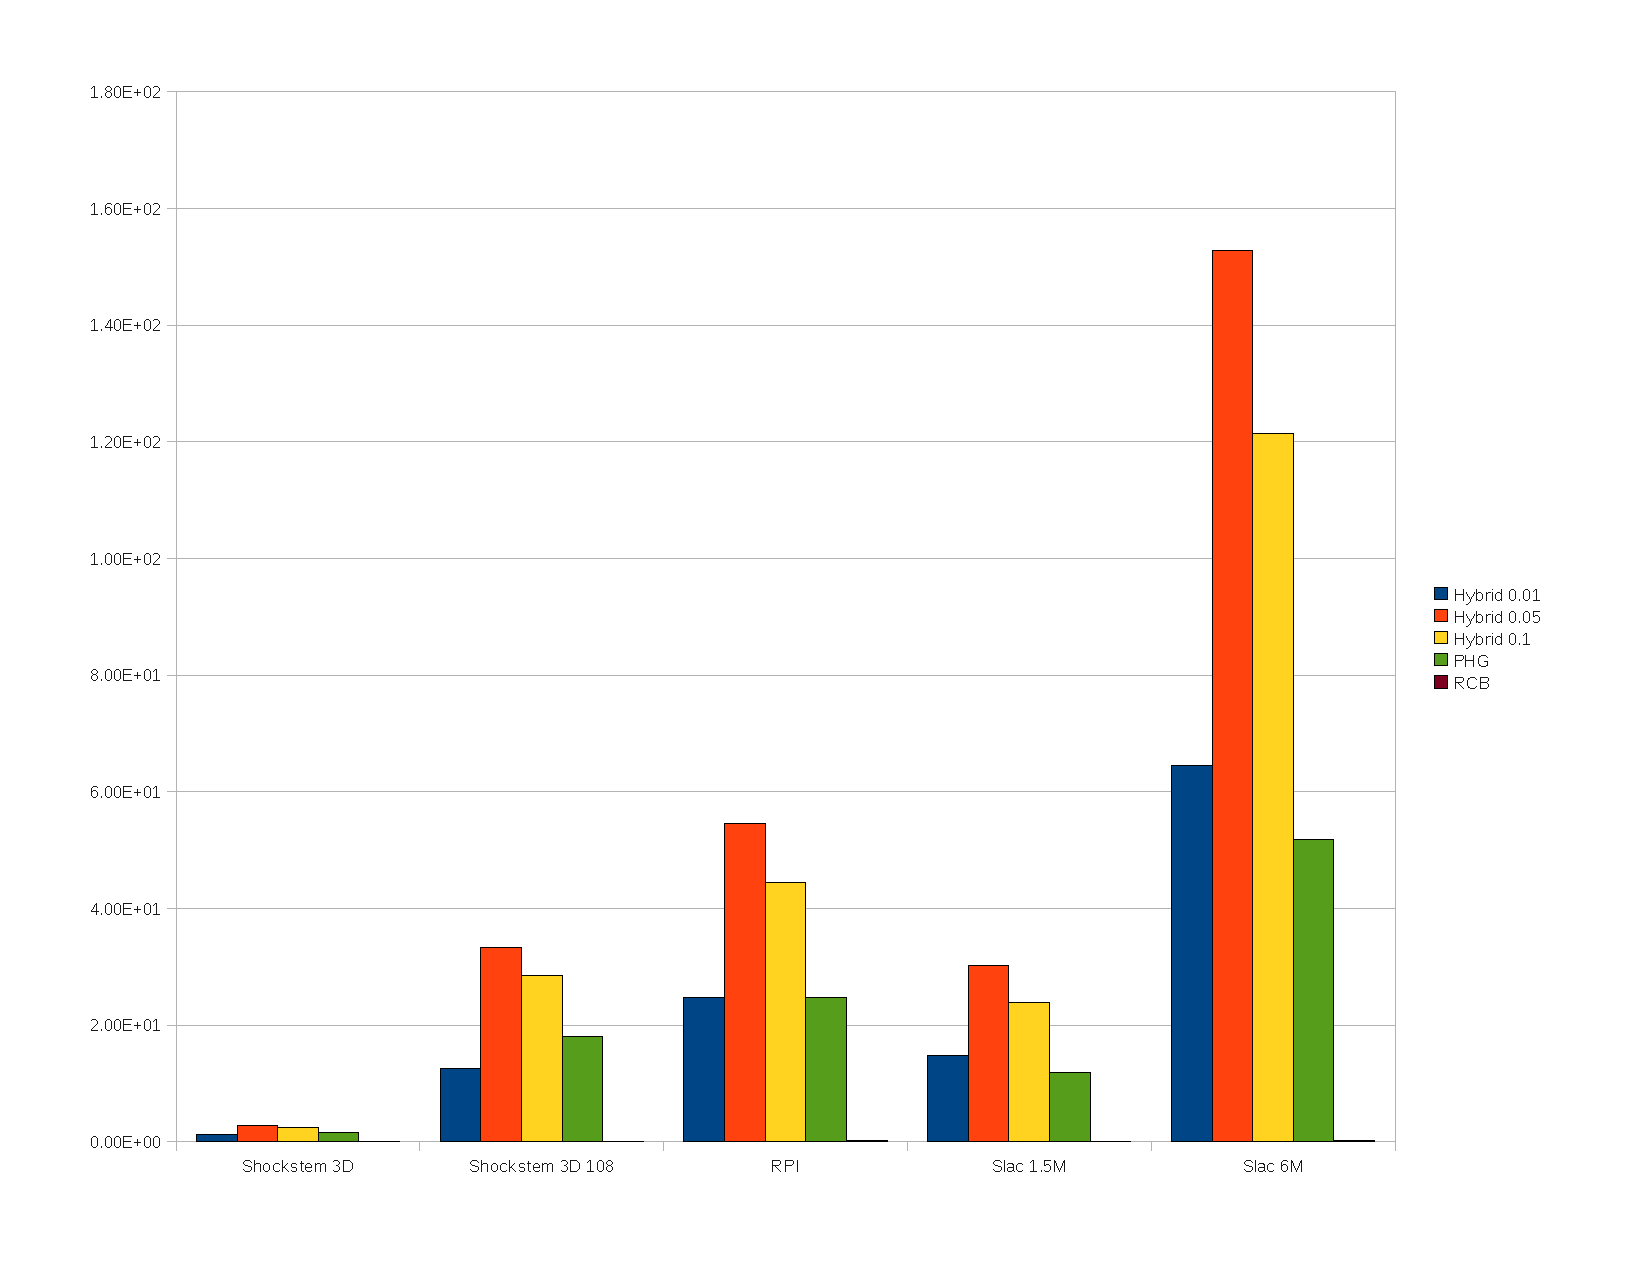
\includegraphics[width=\textwidth, height=80mm]{128_time.pdf}
  \caption{Runtimes on 128 processors}\label{fig:Times_np_128}
\end{figure}



%NEED cutl @ 128 PROCS
\begin{figure}[hgp]
  \centering
  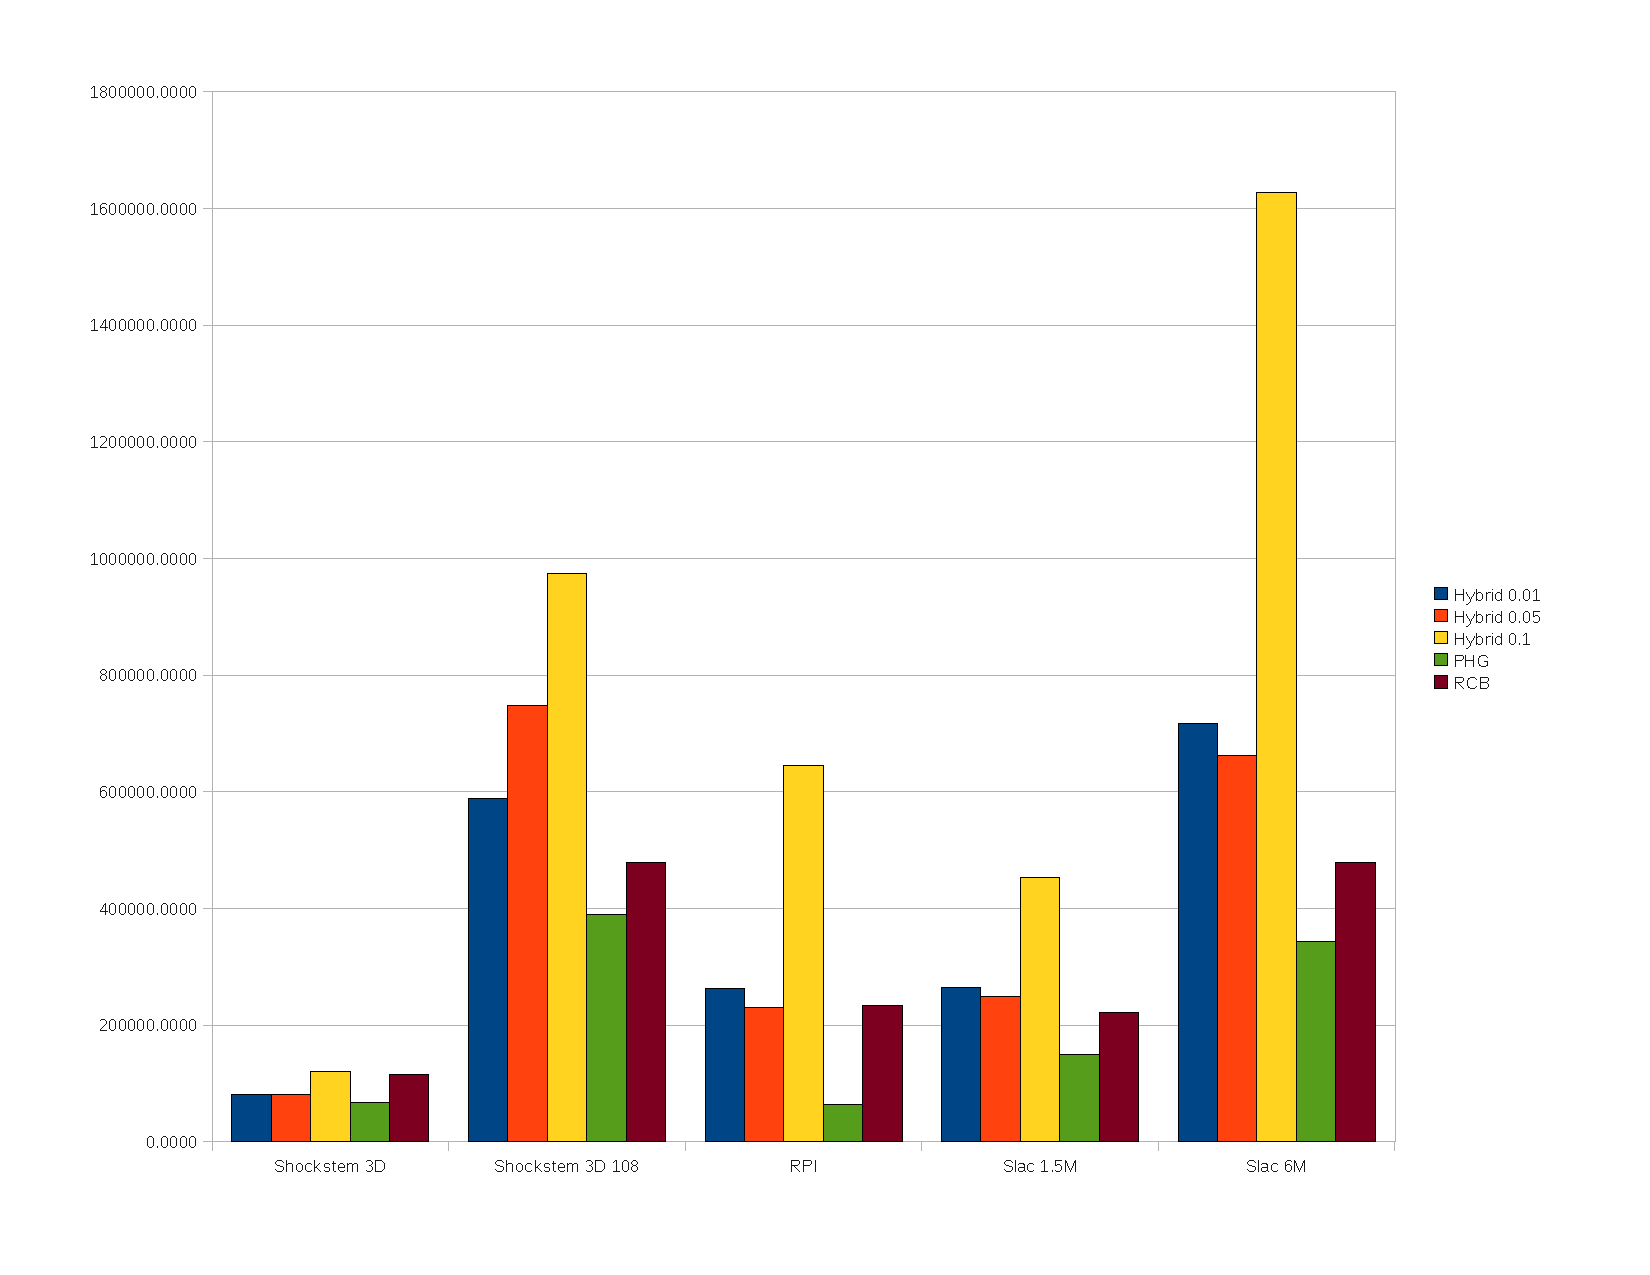
\includegraphics[width=\textwidth, height=70mm]{128_cutl.pdf}
  \caption{Cuts on 128 processors}\label{fig:Cuts_np_128}
\end{figure}

You can see from Figure 1 and 2 that at 128 processors the hybrid methods
are mainly slower than PHG and less accurate than RCB: both results are
the inverse of what we had hoped. There was better news looking at where
the processes were taking their time though:

%timer breakdowns for 128
\begin{figure}[hgp]
  \centering
  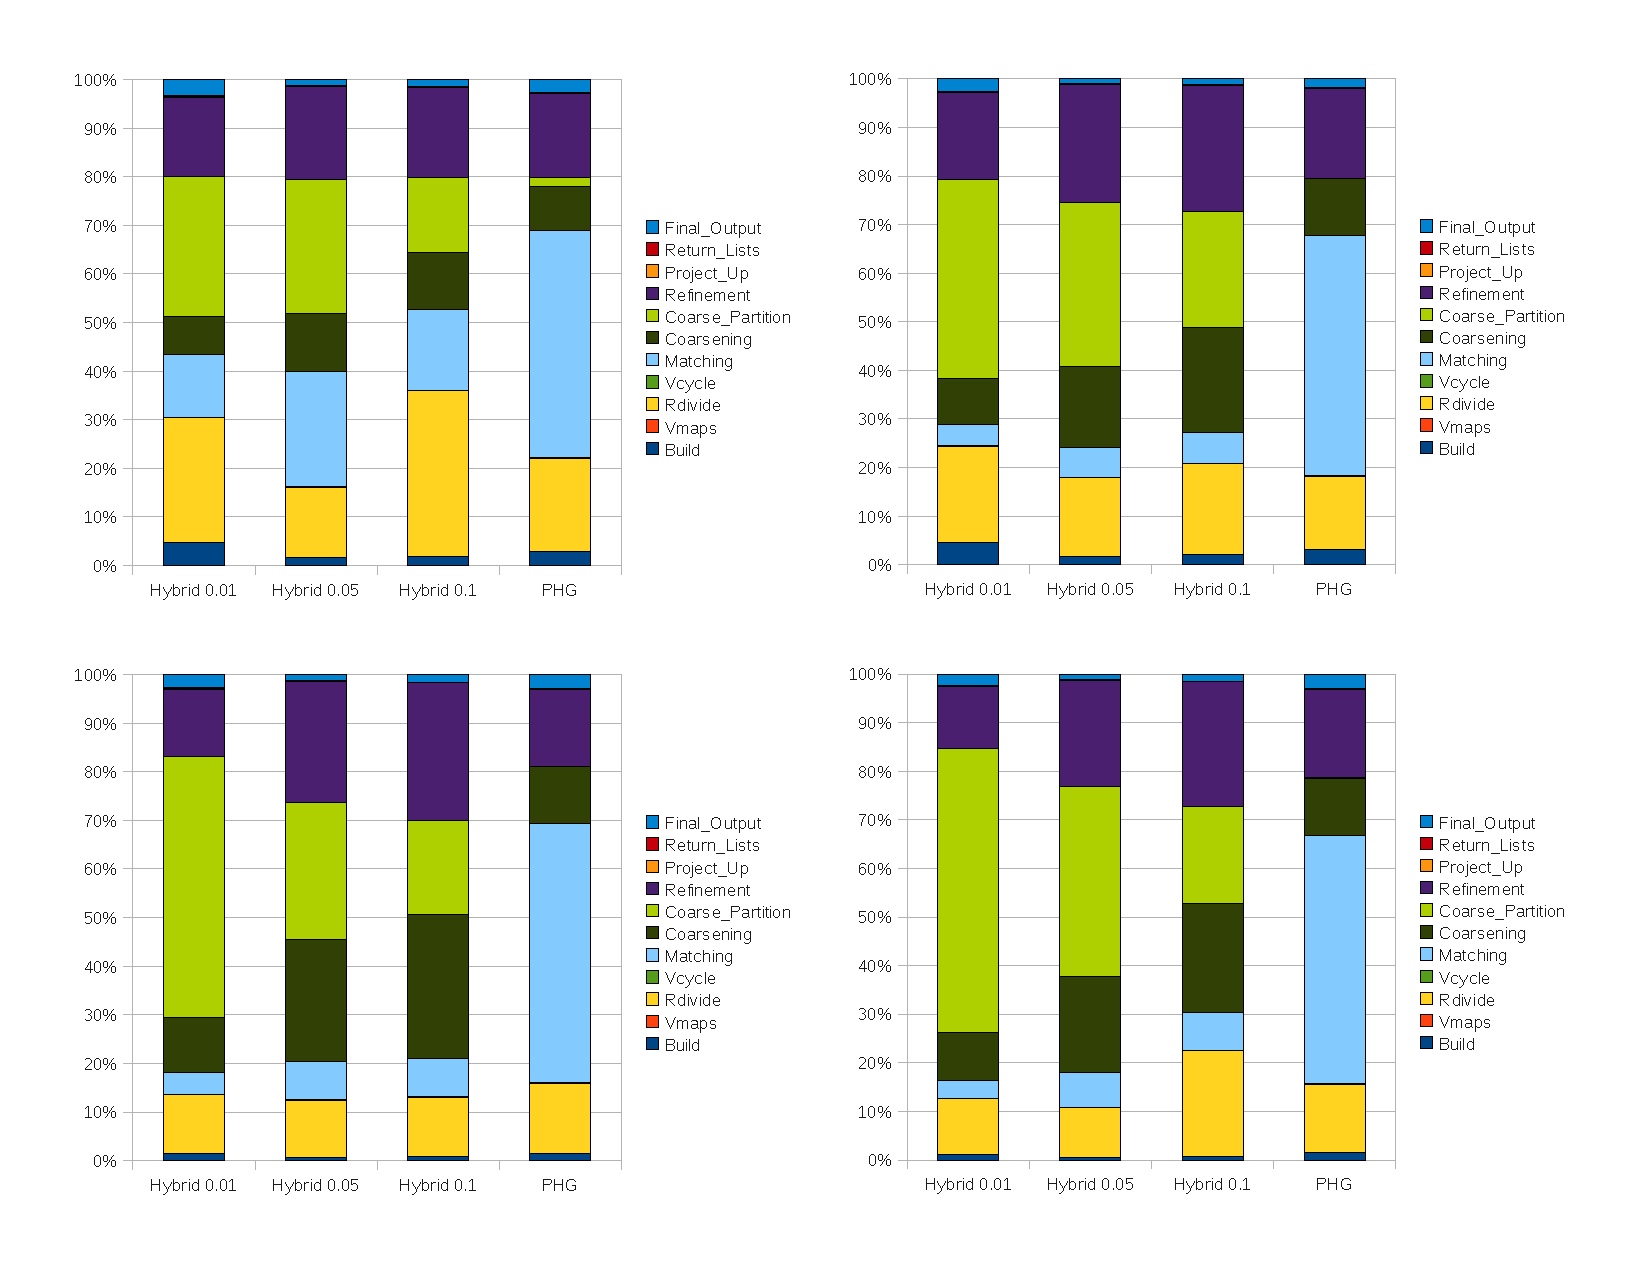
\includegraphics[width=\textwidth, height=70mm]{128_breakdown_percent.pdf}
  \caption{Timing by percentage on 128 processors (UL, Shockstem 3D; UR,
  Shockstem 3D -- 108; LL, RPI; LR, Slac1.5}\label{fig:Percent_np_128}
\end{figure}

The dramatic decrease in the matching time meant that RCB was, indeed,
helping on that front.

When we ran our simulations in serial, however, we saw some very different
results:

%times, cutl
\begin{figure}[hgp]
  \centering
  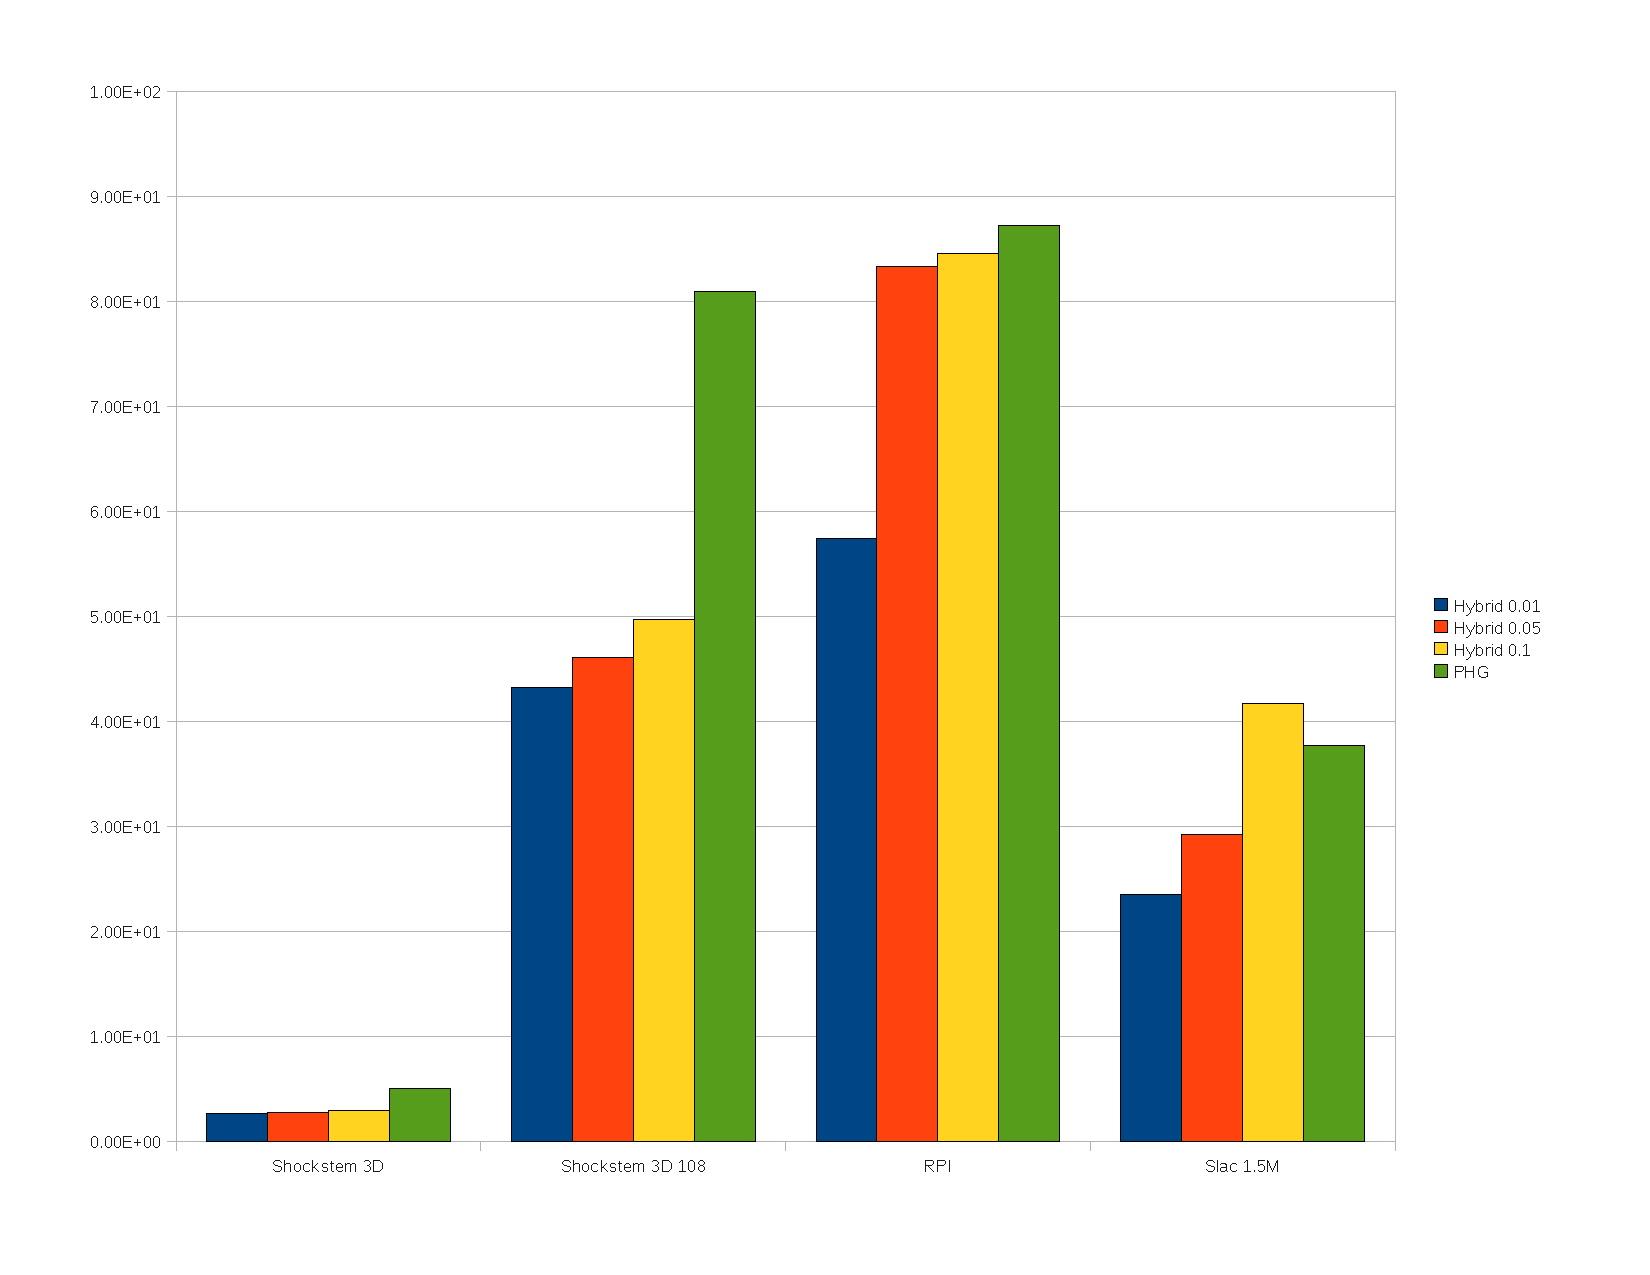
\includegraphics[width=\textwidth, height=80mm]{2_time.pdf}
  \caption{Runtimes in serial on 2 processors}\label{fig:Times_np_2}
\end{figure}



%NEED cutl @ 128 PROCS
\begin{figure}[hgp]
  \centering
  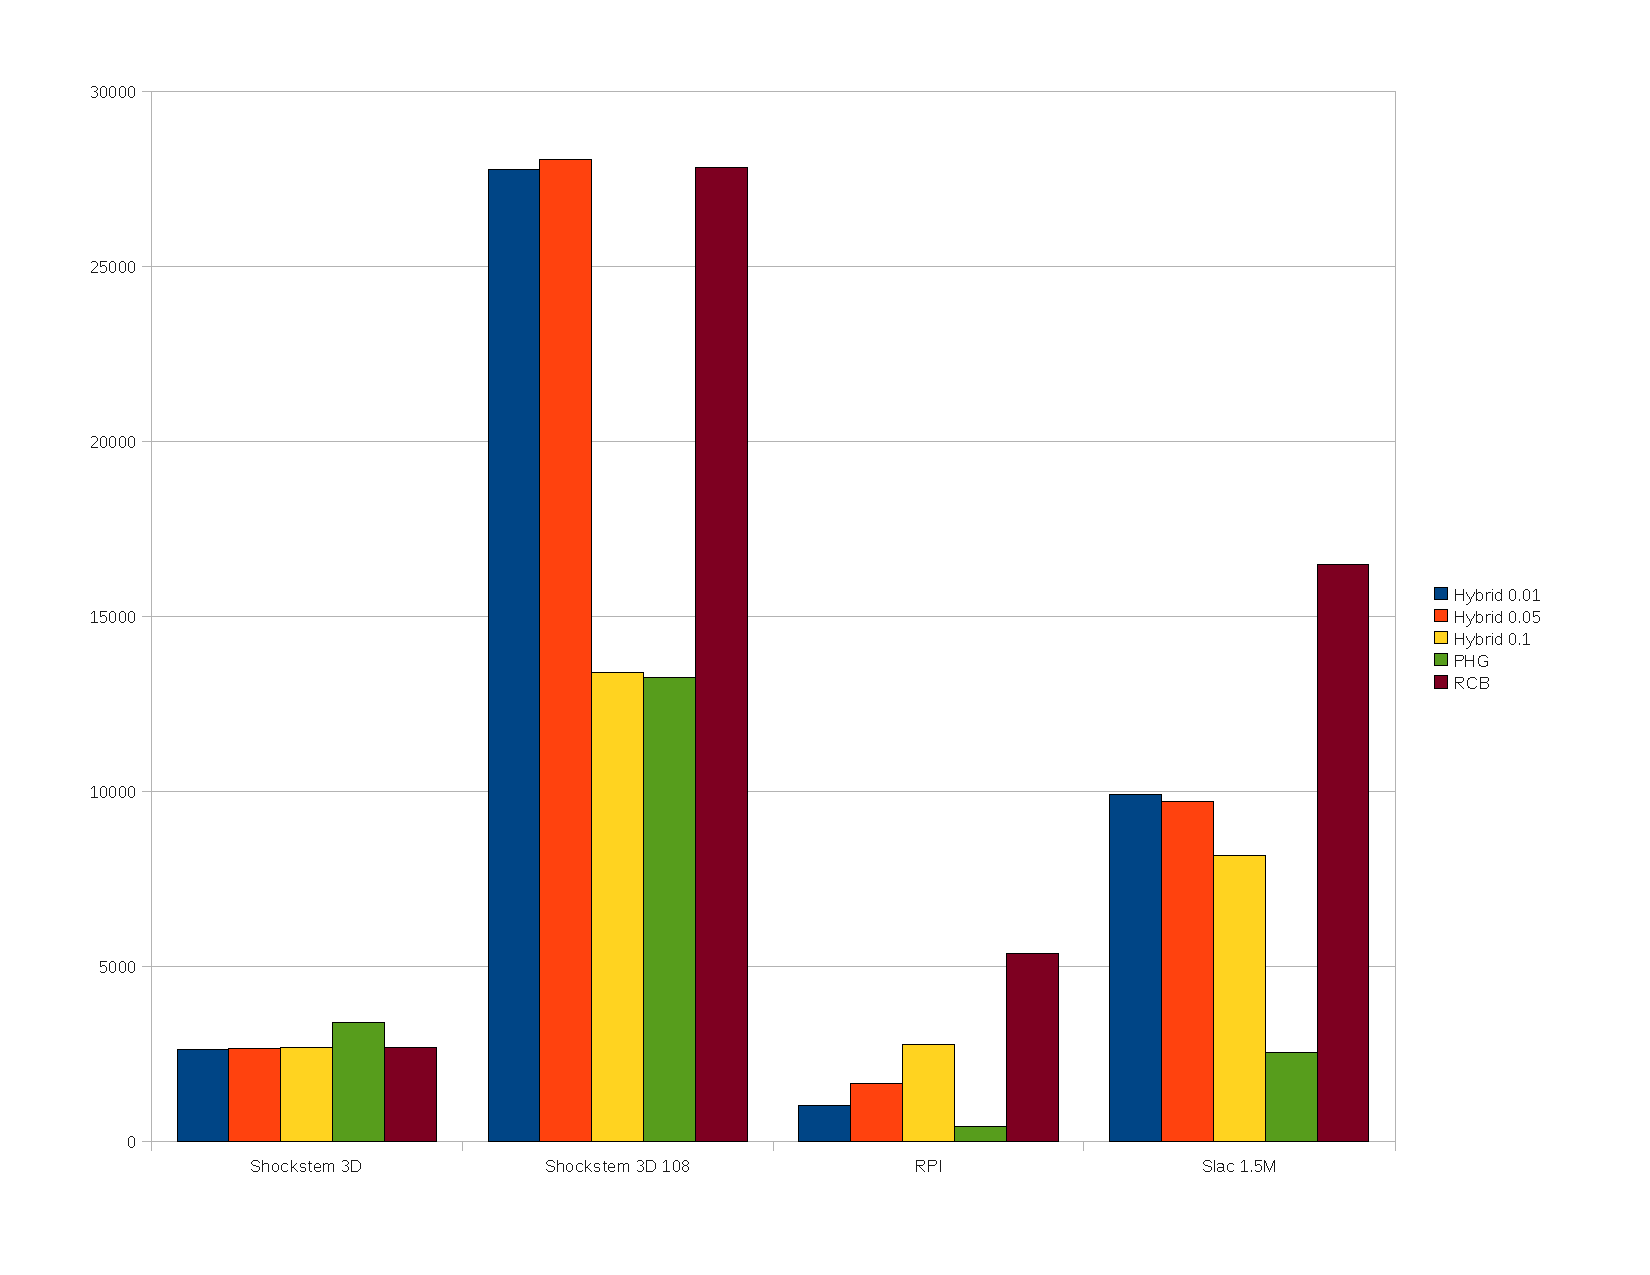
\includegraphics[width=\textwidth, height=70mm]{2_cutl.pdf}
  \caption{Cuts in serial on 2  processors}\label{fig:Cuts_np_2}
\end{figure}

In general the hybrid times beat the PHG times, and the hybrid cuts beat
the RCB cuts.

%time breakdowns for 2
\begin{figure}[hgp]
  \centering
  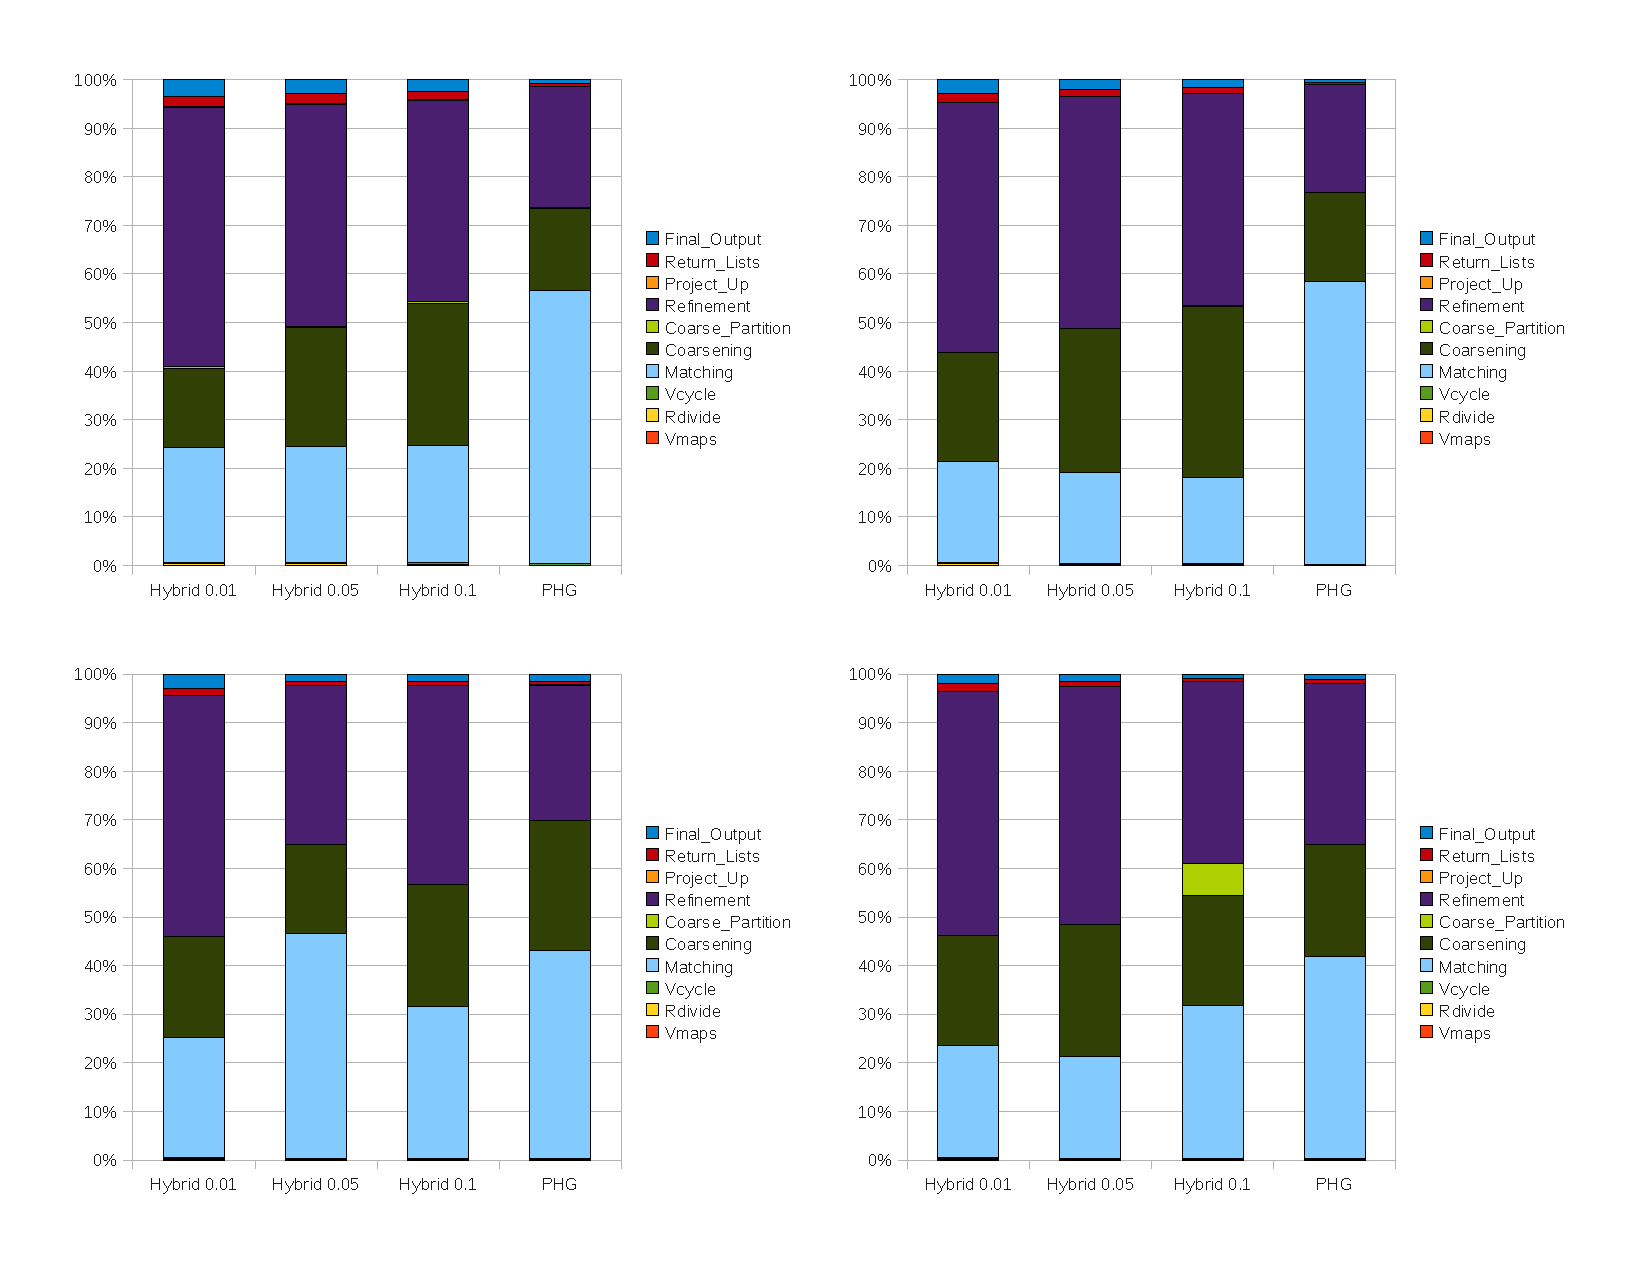
\includegraphics[width=\textwidth, height=70mm]{2_breakdown_percent.pdf}
  \caption{Timing by percentage on 2 processors (UL, Shockstem 3D; UR,
  Shockstem 3D -- 108; LL, RPI; LR, Slac1.5}\label{fig:Percent_np_2}
\end{figure}

Looking at individual timers in this serial run, we can see that RCB has
still drastically reduced the matching time. In addition, the slowdown in
the coarse partitioning has been greatly reduced.

\section{Conclusion and discussion}
The parallel implementation of hybrid partitioning is obviously not
functioning as desired, but we believe that there is ultimately a great
deal of promise in this method. Seeing the results from our serial runs
is encouraging, and it would be worth the effort to continue forward.

Perhaps it would be helpful to check for any communication issues arising
between processors. The whole system could potentially drag, was a
single processor waiting for a message. Additionally, Dr. Catalyurek had
suggested only using RCB-based coarsening on the largest, most complex
hypergraphs, and then revert to standard agglomerative matching for
coarser iterations.

At this moment, there could be four different ways to use Dr. Catalyurek's
method: the first, and perhaps simplest of the three, would be to hardwire
in the number of coarsening levels to give to RCB. A second way would be
to define a new parameter to allow the user to select the number of
RCB-based coarsenings. A third would be to write a short algorithm to
determine and use the optimal number of layers based off of the input.
Finally, there could be an option of user input, with a default to
be either of the other ways.

\begin{thebibliography}{5}

\bibitem{Catalyurek}U.V. Catalyurek, E.G. Boman, K.D. Devine, D. Bozdag,
  R.T. Heaphy, and L.A. Riesen. \emph{A Repartitioning Hypergraph Model
    for Dynamic Load Balancing.} Sandia National Labs, 2009.

\end{thebibliography}

{\small \noindent August 2011.}
\end{document}


